\documentclass{article}
\usepackage[utf8]{inputenc}
\usepackage{graphicx}
\usepackage{float}

\title{Design Document: bike4share}
\author{Maffioli Sara, Papale Lorenzo, \\ Stucchi Lorenzo \& Vaghi Federica}


\begin{document}
\maketitle
\tableofcontents

\newpage

\section{Introduction}

The scope of the “bike4share” Web Application is to guarantee to the user a web service that is able to search for the availability of bikes and free stalls around his position or of the desired location in the city.\\
For the development of the “bike4share” software are required:
\begin{itemize}
    \item PostgresSQL 
    \item Python
    \item Flask
\end{itemize}
 PostgresSQL is used in order to manage the databases, Python is used in order to perform the outputs using the available libraries, such as Shapely, Pandas and Geopandas that are used in order to build the map managing also the background one with the entities that we want to represent while libraries as Bokeh are used for the visualisation of the statistics.

\subsection{Purpose}
This document is a generic Technical Design Document document for “ bike4share”. The purpose of this document is to outline the technical design of the “bike4share” Web Application system and provide an overview for the used databases and software.\\
It is mainly  intended to assist the customer that has invested in sustainable mobility (Municipality of Milan) and the technicians who have to monitor the system in order to work on data and extract the needed informations.
\subsection{Scope}
The final output of the “ bike4share” project will be a client–server computer program which the client, including the user interface and client-side logic, runs in a web browser.\\
The system will allow  the user to interact with a web page in which different functions are offered to different type of users. \\
The basic function are provided to all the users and they consists on:
\begin{itemize}
    \item Showing the position of all the bike stalls
    \item Realtime number of bikes per each stalls
    \item Number of the free stalls for the selected station
\end{itemize}
The premium functions are in addiction of the basic function and they are  accessible for the users after the registration, once the log-in phase is successfully completed, the registered user can access to different functionalities that can help the usability of the app. \\\\\\\\
Premium functions consist on:
\begin{itemize}
    \item Displaying of the position of the user on the map
    \item Help the user to see the nearest station with respect to his position
    \item Showing the list of all the available  stations near the maps
    \item Manually typing of the address or select the position on the map  
    \item Access to statistics
\end{itemize}
A specific section of the application is devoted to the technician’s use. 
The technician is requested to complete the registration and log-in to have access to this specific section in which in addition to all the other functionalities they can perform some  analysis and  graphical statistics with specific tools.
Technician functions consist on:


\begin{itemize}
   \item plotting of the stations median bikes availability per day of the week
   \item plotting of the stations median bikes availability per day of the month
   \item plotting of the total bikes availability per day of the week 
   \item plotting of the total bikes availability per day of the month
\end{itemize}
The main advantages of “bike4share” is the possibility of planning the usage of a bicycle for the daily mobility in a sustainable way, in order to avoid delay, stress and unexpected events while there are important delivery or scheduled appointment.
The main goal is to provide to the customers, users and technician the best services as possible in terms of system performance and functionalities in order to help them with their daily objectives.
Thanks to the premium functionalities it’s possible to avoid different organizational problems. 
Even if the users don’t allow to access to the position because of privacy reasons it’s however possible to use the “bike4share” Web Application thanks to the manual typing of the addresses.  
The log-in and password request are able to reduce the security risks for the users and the main risk related to the usage of this application in case of a security hack will be related to the acquisition of data regarding the positions of the users.
\subsection{Definitions, acronyms and abbreviations}
DB: database\\
DBMS: database management system\\
b4s: bike4share 
\subsection{Document Organization}
This document is organized in different sections like described in Table 1.

\begin{table} [H]
    \begin{center}
        \begin{tabular}{|l|p{0.6\textwidth}|}
            \hline
            Introduction &   Provides information related to this document         \\
            \hline
            Design Overview &  
            Describes the approach, architectural goals and constraints \\
            \hline
            System Architecture &  
            Describes s the various system components and their integration \\
            \hline
            Data Design & Outlines the design of the DBMS and non-DBMS files \\
            \hline
            Detailed Design & Describes the proposed design in detail 
            \\
            \hline
             Human-Machine Interface & Describes the proposed interface
            \\
            \hline
            System Integrity Controls
             & Describes the levels of control
            \\
            \hline
        \end{tabular}
    \end{center}
\label{tab:sec}
\caption{Document organization}
\end{table}

\section{Design Overview}
This section briefly introduce the system context and design, and discuss the background to the project
\subsection{Approach}
The “bike4share” Web Application is created and extended in multiple phases over the course of the project:
\begin{itemize}
    \item Requirements Phase: during this phase the initial version of the documentation is created describing the candidate architecture to be validated in the System Design Phase.
    \item System Design Phase: during this phase the Evolutionary Prototype is created and the documentation is finalized by establishing a sound architectural foundation for the Construction Phase
    \item System Design Phase: during this phase the Evolutionary Prototype is created and the documentation is finalized by establishing a sound architectural foundation for the Construction Phase
    \item Training Phase: during this phase no further additions or modifications are made to the documentation
\end{itemize}

\subsection{Background Information}

The  customer has invested in sustainable mobility by installing a number of bike stalling stations around the City. The implemented bike sharing system must be monitored with the “bike4share” WebApp for assessing the bikes flow both in space and time and, eventually, for designing future system improvement actions. 
Also, the customer has the need to inform in real time bike sharing users about the status of each stations.

\subsection{Constraints}
Technical constraints:
\begin{itemize}
    \item PostgreSQL
    \item Python-Flask 
    \item Python-Bokeh
    \item Python data analysis and plotting
    \item A vector map of the stalling stations (shapefile)
\end{itemize}
Delivery constraints are scheduled as follow:
\begin{itemize}
     \item First version of requirement analysis document	
     \item First version of the Design Document and Test Plan are scheduled on the 26th of May in 2019,
     \item implementation, test report and updated document scheduled on the 09th of June in 2019 
\end{itemize}

\subsection{ Design Trade-offs}
The trade-off method used in the development of the “bike4share” application is based on the functional and quality requirements of the predicted system, a number of scenarios was created in order to  represent both the day-to-day use, and the intended use of the Premium  functionality introduced (ref cap 2.8.1) . 
Using these scenarios, different functional parts are then extracted from architecture descriptions prepared for each of the use-case scenarios. Since the evaluation is conducted at the architecture level, the different parts can  cover measures such as the number of active data repositories, passive data repositories, persistent and non-persistent components, data links, control links, logical groupings, styles and patterns and violations of the intended architecture. These metrics are collected by the developer of the whole system that estimate complexity, impact and effort for each of the scenarios for each of the architectures using an existing architecture as a point of reference (for example the BikeMi services). Based on the collected metrics it is then possible to compare the architecture alternatives and based on that select the most appropriate architecture for the improvement of the system. The alternative architectures are assessed with mainly respect to robustness but they are also compared for reliability, maintainability, interoperability, portability, scalability and performance.

\subsection{User Characteristics}
There are different kind of users but everyone wants to interact with some informations about the bike stalls placed in Milan
\begin{itemize}
    \item Registered user:  a user that is registered yet and that wants to access the “bike4share” WebApp services in order to use the premium functions available  on  the application, it  could  be  a  person  that  uses this service frequently.
    \item Not  registered  user:a user  that  isn’t registered  yet  and  that  wants to ccess  the  “bike4share”  WebApp  services  in  order  to  use the  basic functions available on the application, it could be a person that doesn’t use this service frequently or a new user that wants to start an approach to this service and try it for the first time 
    \item Technician:  a person who is authenticated thanks to specific credential given by the master of the service and who has been granted supervising permissions.   He/she  is  allowed  to  view,  analyze,  access  statistics  and aggregated information about the “bike4share” WebApp services.
\end{itemize}

\subsubsection{User Problem Statement}
In this section the main problems that a user could have by experiencing the “bike4share” WebApp  are described.
It is possible to identify the following problems with respect to the type of event that is occurring .
\begin{enumerate}
    \item User Problem:Registration phase
        \begin{itemize}
            \item Invalid user name: the username exists yet so an error is shown and it is proposed to change the previous username
            \item  Incorrect e-mail address: the format of the mail is wrong so the system requires to correct it and insert a valid one.
    \end{itemize}
    \item User Problem:Log-in phase 
        \begin{itemize}
            \item localization doesn’t work: so the system provides to the logged user the possibility of  manually inserting the needed address and find the position or adding a point in his position.
            \item maps providers crash
            \item server doesn’t work
    \end{itemize}
\end{enumerate}

\section{System Architecture}
Our web application “bike4share” will work thanks to several components supporting it.
We can recognise three levels of the system: User, Software and Data, as is showed in figure \ref{fig:schema}. 
\begin{figure}[h]
    \centering
    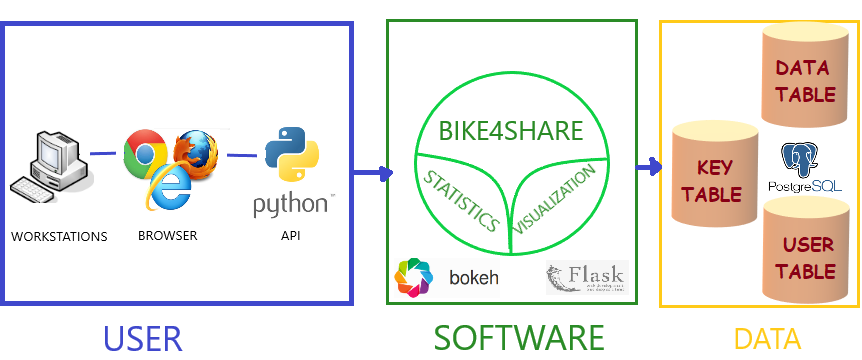
\includegraphics[width=0.75\linewidth]{image/BIKE4SHARE_SCHEMA.png}
    \caption{Overall view of "bike4share" system architecture}
    \label{fig:schema}
\end{figure}
Starting from the bottom and considering the inputs, Data are retrieved from three Databases, one for the registered users and technicians, one for the information regarding the bike stations and one for the secret key created for the first log-in of the technician.
The outputs of “bike4share”, instead, are the visualisation of a map showing the bike stations with the relative information (bikes and free stalls) and the visualisation of statistics (only for technicians and premium users). 
The third level is the one regarding the user, capable of viewing the map to obtain the information, and the technician, who can perform API request to analyse data and statistics. Both the actors can perform their purposes accessing the page through the browser.
\subsection{Hardware Architecture}
As seen in the previous paragraph, the Bike4share is designed as a three-layers architecture but, since the system involve the use of a single machine, the role of all the components is played by the machine itself. So instead of having a distributed system, the hardware architecture is designed as centralized.  A graphical description is shown in the figure \ref{fig:over}.
\begin{figure}[h]
    \centering
    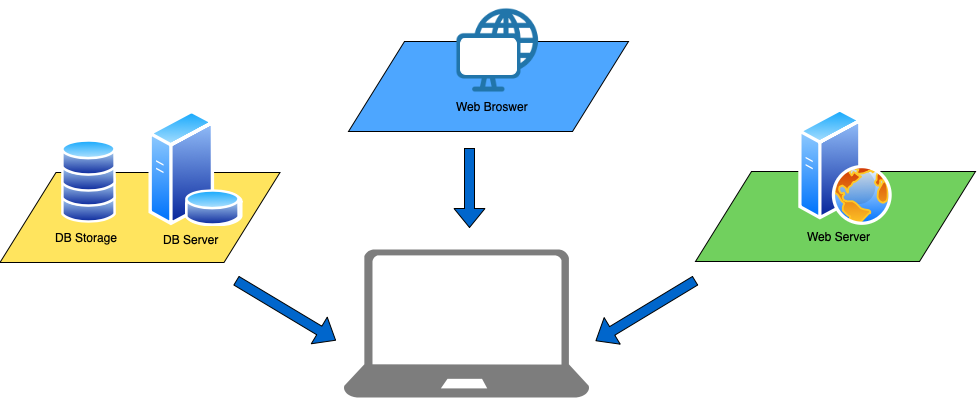
\includegraphics[width=0.55\linewidth]{image/hardware_architecture.png}
    \caption{Overall view of "bike4share" hardware architecture}
    \label{fig:over}
\end{figure}

\begin{itemize}
    \item Database Server: This component, which includes also the DB storage, provides all the data when requested by the application (with SQL queries), allowing it to accomplish its functionalities.
    \item Web Server: It is focused on the workflow and it is responsible for the communication with both the Database Server and the User.
    \item Web Browser: The role of this component is crucial for what concerns the interface, the user informations retrieval (for registration and login) and the presentation of the informations needed by the User and by the Technician. 
\end{itemize}
It is important to consider the fact that changes in the architecture are planned. The system, which works on one machine, will be splitted on three physical layers corresponding to the one described in the previous paragraph and showed in the figure \ref{fig:com_createSchema}.\\
\begin{figure}[h]
    \centering
    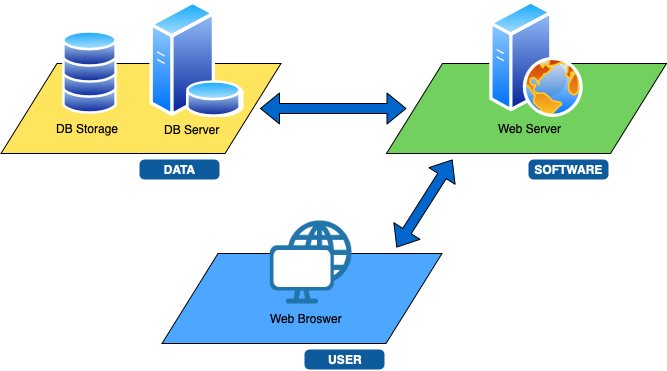
\includegraphics[width=0.85\linewidth]{image/hardware_COMPLETE.png}
    \caption{Communication diagram related to the createSchema module}
    \label{fig:com_createSchema}
\end{figure}

\subsection{Software Architecture}
The software architecture is mainly based on the implementation of the statistics thanks to bokeh and the visualization of the obtained results trough flask.
The programming language is Python and in particular the libraries and the tools that are used are:
\begin{itemize}
    \item Pandas:it provides high-performance, easy-to-use data structures and data analysis tools for the Python programming language. 
    \item GeoPandas:It combines the capabilities of pandas and shapely, providing geospatial operations in pandas and a high-level interface to multiple geometries to shapely random function
    \item Psycopg2:it is the most popular PostgreSQL DB adapter for the Python programming language. It was designed for heavily multi-threaded applications. It features client-side and server-side cursors, asynchronous communication and notifications, many Python types are supported out-of-the-box and adapted to matching  PostgreSQL data types; adaptation can be extended and customized thanks to a flexible objects adaptation system.
    \item Sqlalchemy:it is the Python SQL toolkit and Object Relational Mapper that gives application developers the full power and flexibility of SQL. It provides a full suite of well known enterprise-level persistence patterns, designed for efficient and high-performing database access, adapted into a simple and Pythonic domain language.
    \item Geoalchemy2:it provides extensions to SQLAlchemy for working with spatial DBs and it is focused on PostGIS.
    \item GeoJSON: is a format for encoding a variety of geographic data structures that supports the following geometry types: Point, LineString, Polygon, MultiPoint, MultiLineString, and MultiPolygon. Geometric objects with additional properties are Feature objects. Sets of features are contained by FeatureCollection objects.
    \item Bokeh:it is an interactive visualization library its goal is to provide elegant, concise construction of versatile graphics, and to extend this capability with high-performance interactivity over very large or streaming datasets
    \item Flask:it is a micro web framework written in Python that supports extensions that can add application features as if they were implemented in Flask itself. Extensions exist for object-relational mappers, form validation, upload handling, various open authentication technologies and several common framework related tools. 
    \item PgAdmin: it is a management tool for PostgreSQL and derivative relational databases such as EnterpriseDB's EDB Advanced Server.
    \item Leaflet: it is the leading open-source JavaScript library for mobile-friendly interactive maps, it has all the mapping features most developers need.It works efficiently across all major desktop and mobile platforms, can be extended with lots of plugins and it is an easy to use  API. 
\end{itemize}
The structure of the software is based on the following python schemas and reusable functions:
\begin{itemize}
    \item createSchema: it allows the creation of the different table used by the  “bike4share” WebApp. Thanks to the SQL query and the pgAdmin DBs connection it is possible to access, create, updated, extract data and fill the different DBs which interact with the user side in order to guarantee the consistency with the latest version of the data.
    \begin{itemize}
         \item Key\_generator: it is a function defined in order to automatically generate some random password that will be given to the technician directly from their chief or by our customer (the buyer of the system, the Municipality of Milan)
    \end{itemize}
    \item Webpage:it is the main part of “bike4share”software development, it allows to log-in, access,register, make some statistics and visualize the map in which the bike and stalls information thanks to the direct connection to the DBs with the following main function:
     \begin{itemize}
         \item get\_dbConn: it allows the connection with the  DBs
         \item close\_dbConn: it allows the disconnection from the  DBs
         \item Load\_logged\_in\_user: it allows to check if the user is inserted yet in the user’s DB and make the consequent operations
         \item Index: it allows the map visualization
         \item Register: it allows the registration of the user
         \item Log\_in: it allows the log-in of the pre-registered users
         \item Log\_out: it allows the log-out of the users 
         \item Tech\_reg: it allows the registration of the user
         \item Bash\_command: it allows the bokeh application running on port 5006 to be accessed at port 5000 by Flask
         \item Statistics: it allows Flash to read what is the bokeh server and to have access to the statistics
     \end{itemize}
     \item Statistics: it is the section of “bike4share”software development that  allows to creation of plots, representing the different evaluated statistics. The principal functions are:
     \begin{itemize}
          \item pd.to\_datetime: Pandas function to convert string date time into Python date time object
          \item df\_bike.groupby: it allows to split the data into groups based on some criteria
          \item ColumnDataSource: it allows to store the data to use in the bokeh graph
          \item figure: it allows to create a new figure in Bokeh
          \item callback: it allows to upload the graph 
     \end{itemize}
\end{itemize}

      
\subsection{Communications Architecture}
The Communication diagram, fig \ref{fig:createSchema}, is a diagram that shows the interactions between elements at run-time. They  are used to visualize inter-object relationships.

\begin{figure}[h]
    \centering
    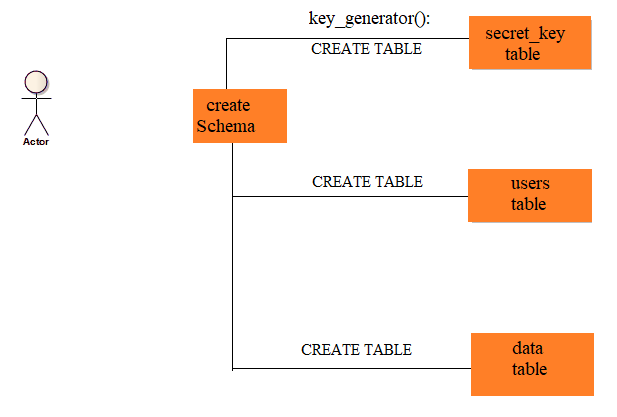
\includegraphics[width=0.75\linewidth]{image/COMM_TAB.png}
    \caption{Communication diagram related to the createSchema module}
    \label{fig:createSchema}
\end{figure}

\begin{figure}[H]
    \centering
    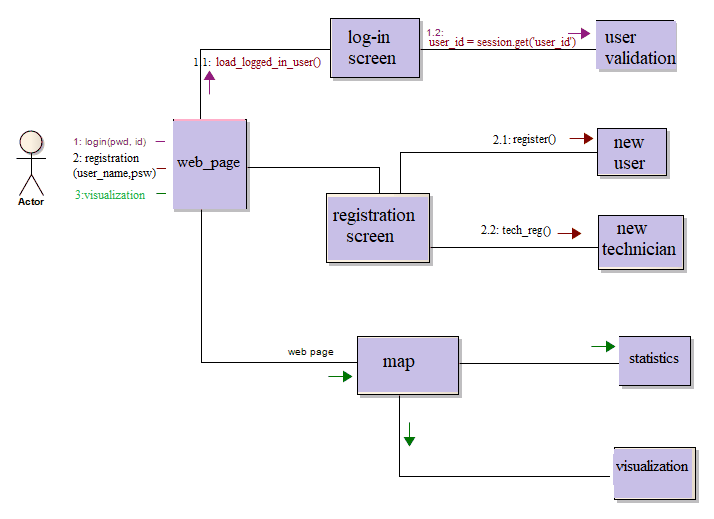
\includegraphics[width=0.75\linewidth]{image/comunication_architecture.png}
    \caption{Communication diagram related to the webpage module}
    \label{fig:webpage}
\end{figure}

The schema in fig. \ref{fig:createSchema} is possible to notice how the createSchema python code is linked with the DB and how it can interact in the creation, modification and update of the dataframes.

In the figure \ref{fig:webpage} is possible to see how the different modules of the “bike4share” application are linked and how they interact between themselves. This schema isn’t complete yet but it represents the main communication architecture of the web\_page software schema of the application.

\section{Data Design}
The DBMS chosen for this purpose is PgAdmin4 and the DB is mainly composed by 3 tables:
\begin{itemize}
\item Key\_list table: this table contains the random generated passwords for the first registration of the technician,once that one of those password is been used it’ll be deleted 
\item User\_bike table: this table contains the credentials of all the registered users in order to allow them to perform the log-in procedure. It’s checked, filled and updated every time that a new user try to make the registration
\item Stations:this table contains the all the initial given data regarding:
 \begin{itemize}
 \item bike availability
 \item number of stations
 \end{itemize}
\end{itemize}

\subsection{Database Management System Files}
In this section will be described how the DB will be designed 

\begin{figure}[h]
    \centering
    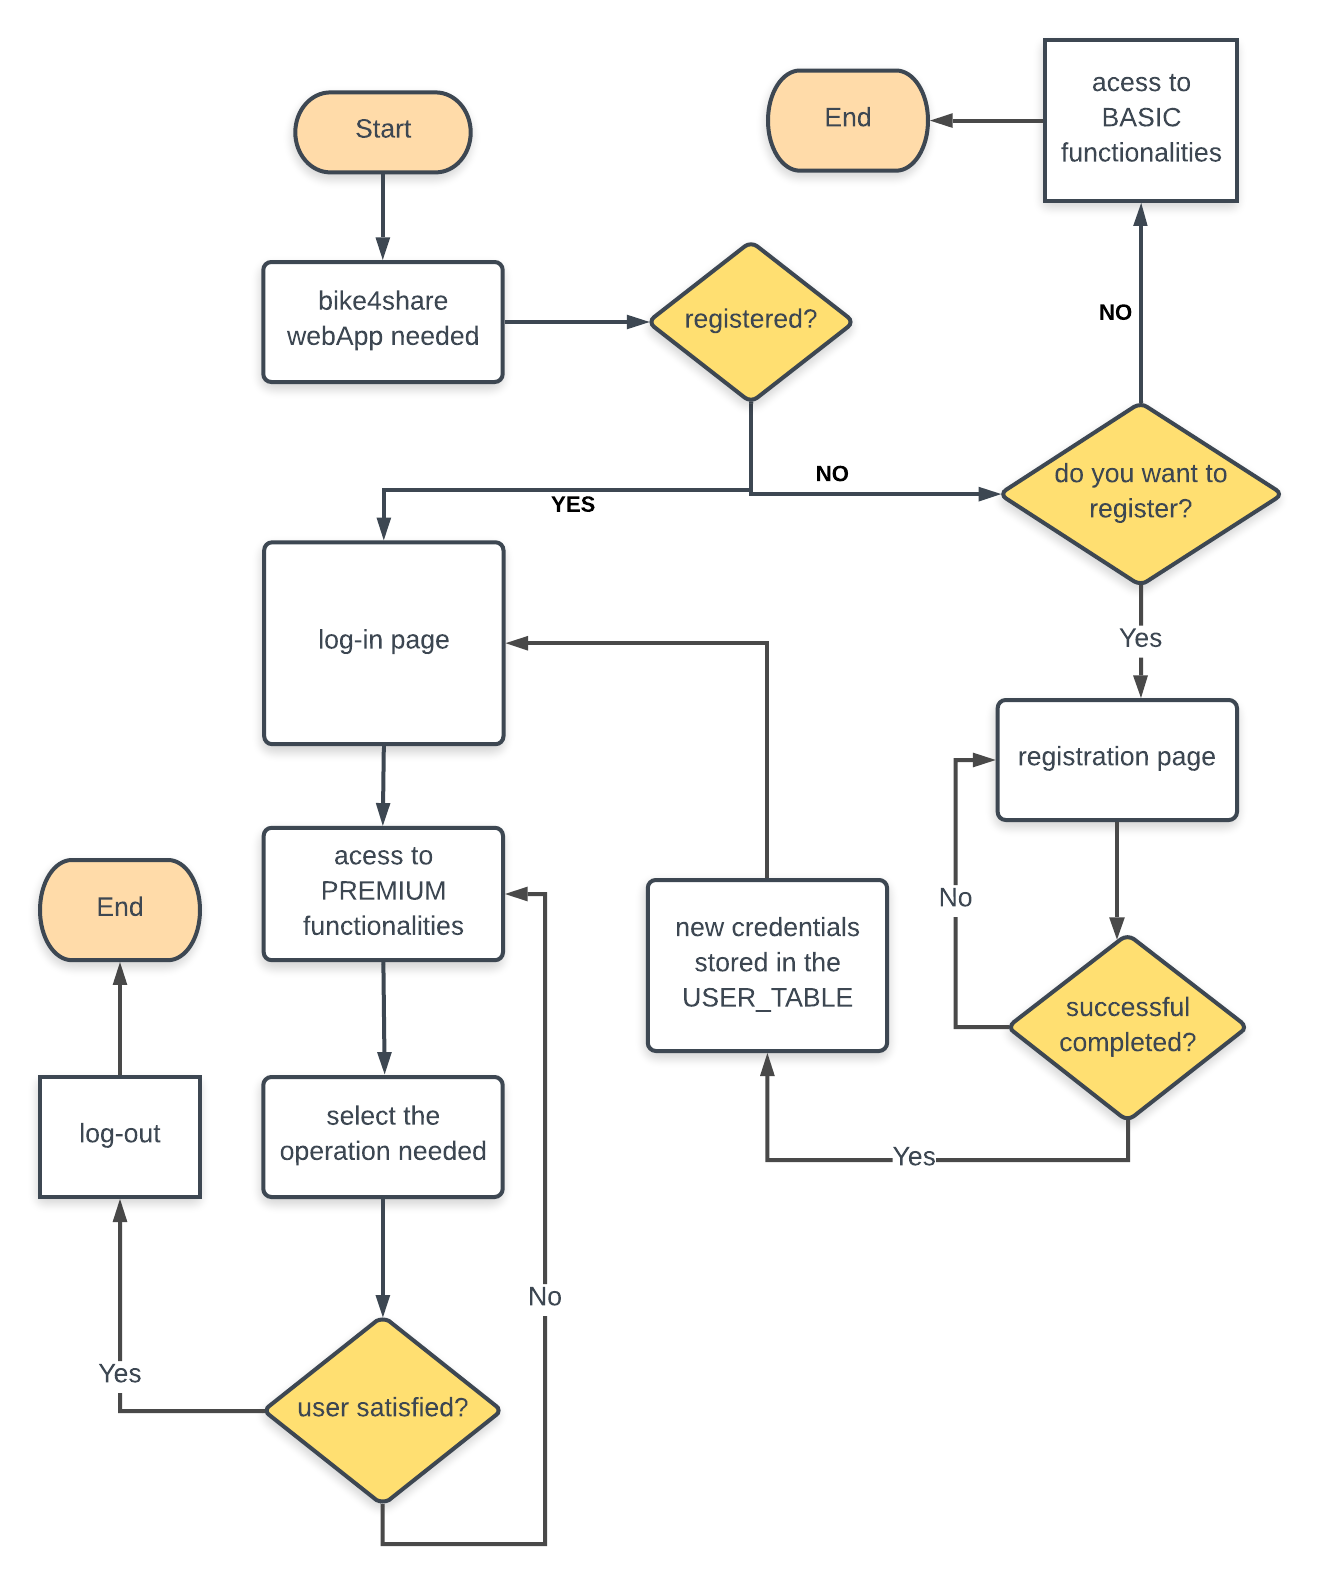
\includegraphics[width=0.55\linewidth]{image/flow_chart.png}
    \caption{Representation of the flow of the events related to the usage of the b4s}
    \label{fig:flow}
\end{figure}

The Table 2 will show the main attributes that describe the DB tables.

\begin{table} [H]
\begin{tabular}{|l|p{0.18\textwidth}|l|p{0.12\textwidth}|p{0.12\textwidth}|}
 \hline TABLE NAME &   TABLE COMMENTS &    COLUMN NAME & DATA TYPE & DATA LENGTH    \\
 \hline
 KEY\_LIST &  Random technician passwords & Id\_key &int(PK)& -\\
  & &  secret\_key & varchar & 35\\
 \hline
 STATIONS  &   Informations regarding stations & ID &int & -\\
  & &  BIKE\_SH & text & - \\
  & & INDIRIZZO & text & - \\
  & & STALLI & int & - \\
  & & LOCALIZ & text & - \\
  & & LATITUDINE & double & - \\
  & & LONGITUDINE & double & - \\
 \hline
 USER\_BIKE &  Informations regarding users & user\_id & int(PK)& -\\
 & & user\_name & varchar & 255 \\
 & & user\_password & varchar & 255 \\
 & & user\_type & varchar & 255\\
 \hline
\end{tabular}
\label{tab:attributes}
\caption{Database structure}
\end{table}

\section{Detailed Design}
\subsection{Software Detailed Design}
In this section the different module composing the “bike4share” web app will be described and commented.

\subsubsection{Module 1: CreateSchema}
In this module it is possible to create the different table stored in the DB.
\paragraph{CreateSchema: Processing}
The first operation that is made in this module is the dropping of the existing table in order to avoid inconsistency of data. After that it’s possible to create the tables (key\_list, user\_bike) with all the needed parameters.
\begin{figure}[H]
    \centering
    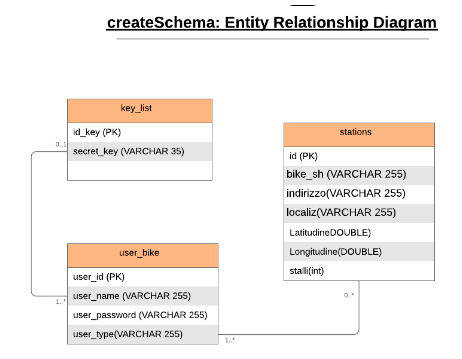
\includegraphics[width=0.55\linewidth]{image/schema_entity_relationship.png}
    \caption{Schema entity relationship between the databases}
    \label{fig:relationdb}
\end{figure}
The key\_list table is filled thanks to the function key\_generator() that is able to generate different random password composed by chars, numbers and special characters value for a defined number of time; in this way is possible to check the quantity of allowed technician and to check if their password are used yet.
The described tables are linked with the stations table that is generated, filled and modified thanks to another module called "downloadStation". 

\paragraph{Local data structures}
The main structures used to store data are data frames.

\subsubsection{Module 2: downloadStation}
This module is used to download the data of the stations directly from the server , it is automated and it’s imported by the webpage module. It refers to the bike.csv input data file.
\paragraph{downloadStation: Processing}
It implies the creation of  a separate geojson file from the webpage module, it is based on the usage of the function data2geojson()  that allows to georeference the points of the stations with respect to the coordinates and the reference system used in the map. The function data\_to\_geojson() allows to make the connection between the DB in which the table of the stations is available.

\subsubsection{Module 3: webpage}
This module is the main module of the “bike4share” system used to create the general schema of the website in order to connect the different sections: map, login, logout, registration and statistics.
\paragraph{webpage: Processing}
The first point consists in the creation of the application instance. Then different functions are implemented to establish the connection with the DB such as get\_dbConn() and close\_dbConn(). The different sections are connected through the following functions:
\begin{itemize}
    \item load\_logged\_in\_user()
    \item index()
    \item register()
    \item login()
    \item logout()
    \item tec\_reg()
    \item Bash\_command
    \item statistics()
\end{itemize}

All the URLs are defined as routes in the Flask application through the app.route decorator. 
\paragraph{webpage: Local data structures}
The main structures used to store data are data frames and lists.

\subsubsection{Module 4: statistics}
The aim of  this module is to create different statistics on the base of the data retrieved by the DB, from tables ‘bike\_stalls’ and ‘stations’.
\paragraph{statistics: Processing}
The first operation that is made in this module is the connection to the DB in order to store the tables, above mentioned,  of the data from the database in order to store them respectively in two different data frames. In this way is possible to extract the information needed to compute statistics, e.g. day and month. The data can be stored in data frames using the function df\_bike.groupby on the base of the different criteria as the median and the total availability of bikes. Using Bokeh functions it is possible to plot these statistics and to design the relative widgets. 
\paragraph{statistics: Local data structures}
The main structures used to store data are data frames and lists.
\section{Human-Machine Interface}
The user interface is easy and intuitive, fig \ref{fig:usageb4s}. When the webpage is opened, a map appears on the screen. The map shows the bike stations (as markers) in terms of position in space, with the possibility to interact with it; clicking on them, the user can immediately know what is the address and the capacity (total number of stalls)
\\
\begin{figure}[H]
    \centering
    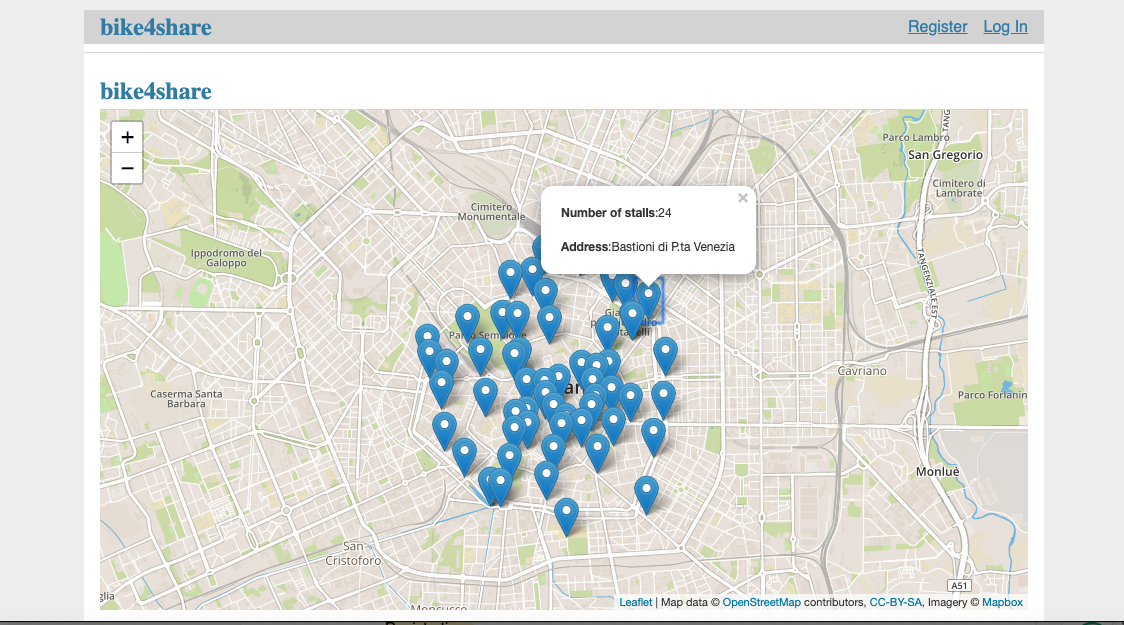
\includegraphics[width=0.8\linewidth]{image/map.png}
    \caption{Rapresentation of the flow of the events related to the usage of the b4s}
    \label{fig:usageb4s}
\end{figure}

\subsection{Interface Design Rules}
As design rule, the webpage is provided with the constant presence of the navigation bar on the top of the page, fig \ref{fig:navbar}. The navigation bar contains the buttons:
\begin{itemize}
    \item BikeE4share (returning the homepage)
    \item Login
    \item Registration
    \item Logout
\end{itemize}
This design rule can help the user in navigating on the webpage with the possibility to return to the home page if something goes wrong.

\begin{figure}[H]
    \centering
    
\includegraphics[width=1\linewidth]{image/navbar.png}
    \caption{Detail representing the navigation bar}
    \label{fig:navbar}
\end{figure}

\subsection{Inputs}
For what concerning the standard users, inputs are not required; the user accesses the Webapp and he can play with the map. 
For technicians and premium users, instead, some inputs are required. For what concerning the registration procedure, premium users have to provide an username and a password; these data will be stored in the DB (the password will be hashed for security purpose). Technicians, in addition, have to fill a specific form with a secret key provided by the company. 
During the login both of them have to fill a form with their username and password. These credentials will be checked in the DB.
\subsection{Outputs}
The webapp provides several outputs, based on the type of user who is logged in.
\begin{itemize}
    \item Standard user: The output provided by the webapp is a map showing the bike stations. The user is allowed to know the address of each station and it's capacity.
    \item Premium user : for this type of user, exists the possibility to automatically locate himself. The map, indeed, shows the position of the user and the stations. In addition, the page contains also some useful statistics designed for the user.
    \item Technician: The technician page contains the same map provided to the premium users, plus a set of statistics (well described in the previous paragraphs).
\end{itemize}

\subsection{Navigation Hierarchy}
In this section is possible to find a diagram, fig \ref{fig:navigation}, of the navigation hierarchy where is shown how a user can move through the interfaces.\\
\begin{figure}[H]
    \centering
    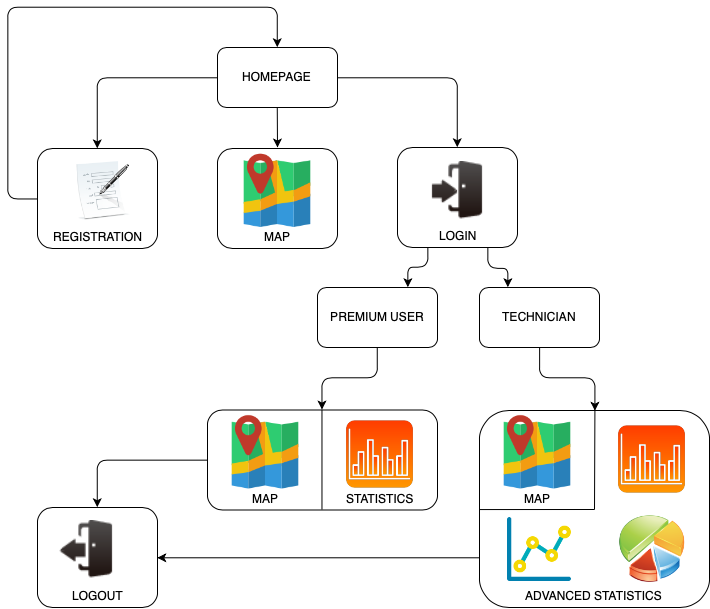
\includegraphics[width=1\linewidth]{image/USERFLOW.png}
    \caption{Diagram of the navigation hierarchy}
    \label{fig:navigation}
\end{figure}

\end{document}